\documentclass[main.tex]{subfile}
\begin{document}
\section{Delopgave 3\\\normalsize{-- Producer-Consumer med bounded buffer.}}
Formålet med denne delopgave er at demonstrer vores vores kenskab til tælle-semafore samt deres anvendelse i praksis. Opgaver bassere sig på et producent/forbruger system, hvor en gruppe producenter generere en række produkter som en gruppe forbrugere benytter.\\

Løsningen til denne delopgave er implementeret i filen \texttt{002\_3.c} og gør brug af implementation af den hægtede liste fra delopgave 2, se afsnit~\ref{sec:opg2} side~\pageref{sec:opg2}.

\subsection{Implementationen, overordnet set}
Implementationen basere sig på at en grupppe producent-tråde, af typen \texttt{pthread\_t}, oprettes sammen med en gruppe forbruger-tråde. Når producent-trådene er oprette begynder de hver især at prodcere elementer og tilføje disse til en fælles buffer. Bufferen er en hægtet liste fra delopgave 2, som forbruger-trådene læser elementer ud af, efterhånden som de bliver produceret. Gruppernes størrelse, bufferens kapacitet samt mængden af elementer der skal produceres er baseret på brugerinput, som gives med når programmet startes.\\

For at sikre at trådene ikke foresager \texttt{race-conditions} gør vi brug af en række binære tælle semafore, som har tilformål at låse forskellige data felter således at kun en tråd kan have adgang til dette ad gangen. Derudover bruger vi også tælle semafore til sikre at bufferens kapacitet ikke overskrides.\\

Når det angivne antal produkter er produceret og et tilsvarende antal er forbrugt at forbruger-trådene skriver programmet en status meddelelse til terminalen, hvorefter programet terminere. 

\subsection{De specifikke løsninger}
\subsubsection{Producenter}
Producent funktionen er implementeret med en \texttt{while-løkke} som bliver køre så længe der skal produceres nye elementer. Til at finde ud af om der skal produceres flere elementer tjekker tråden hvor mange elementer der er produceret, samt hvor mange der ligger i bufferen og sikre sig at summen af disse to tal ikke overstiger den totale mænge af elementer der skal produceres. Hvis alle elementer er produceret bryder tråden ud af løkken og lukker ned.\\

Det første der sker inde i løkken er at tråden sættes til at vente i omkring 1 sekund. Herefter øger den 

\subsubsection{Forbrugere}


\subsubsection{Tælle semafore}
Vi bruger tælle semafore flere steder i vores system. Først og fremmest bruger vi en binær tælle semafor til at sikre at kun en tråd har adgang til bufferen ad gangen. Dette er for at sikre mod race-conditions, hvor flere tråde forsøger at tilføje eller fjerne elementer samtidig. På samme måde gør vi brug af binære tælle semafore til at sikre at der ikke er flere tråde som forsøger at opdatere antallet af producerede/brugte elementer samtidigt. Alt i alt har bruer vi fire binære semafore til at forebygge race-conditions.\\

Udover de nævnte semafore bruger vi yderligere to tælle semafore til at holde styr på henholds vis hvor mange elementer der er i bufferen, samt hvor mange flere elementer der er plads til. 
Hvergang en producent forsøger at tilføje et element til bufferen skal den først reducere værdien på den semafor som hold styr på antallet af tomme pladser i bufferen med én. Hvis denne har værdien 0 må tråden vente på at en forbruger-tråd læser et element ud fra bufferen og hæver værdien af tomme pladser med en. Nå prducent-tråden har tilføjet elementet til bufferen øger den værdien for den semafor som holder styr på antallet af elementer i bufferen. På tilsvarende vis skal en forbruger-tråd reducere semaforen der holder antallet af elementer inden den kan få lov at fjerne et. Er værdien af denne 0 må tråden vente til den kan får en værdi der er større.

\subsection{Fejl og mangler}
Hvis programmet startes med mindre end de fire krævede argumenter vil det terminere med en segmentfejl. Dette er hverken en særlig køn eller bruger venlig løsning da en bruger, som ikke kender systemet hurtigt vil kunne få en opfattelse af at det ikke virker efter hensigten. Her ville det have klædt programmet at det var implementret således at hvis der blev givet for få eller for mange parameter med ved opstarte ville systemet printe en besked til brugeren of enventuelt bede om at få specificeret input parameterne. 

\subsection{Test}
For at teste at programmet virker som forventet har vi kørt den en række gange med forskellige input.
\begin{description}
\item[Store input:] En af de måder hvorpå vi har testet systemet er ved at sætte det til at producere en stor mængde prdukter og kontrolleret at systemet ikke fejler over tid. 
\item[Flest producenter:] Vi har også test systemet ved at køre de med indstillinger hvor der har været væsenligt flere prducenter end forbrugerer og omvendt. Ved disse test har vi haft fokus på at bufferens kapacitet ikke overskrides samt at den type tråde som er i overtal ikke begynder at lukke ned før end at alle elementer er produceret/forbrugt.
\item[For mange producenter:] En tredje måde vi har test systemet på er ved at lave flere producenter end der skulle gennereres elementer. Her har vores fokus været at der kun blev genereret det antal elementer der skulle produceres og at de overflødige producenter ikke producerer noget.
\item[Negative input:] Den sidste måde hvorpå vi har teste vores system er ved at angive negative værdier. Her har formålet været at sikre at systemet håndtere dårlige bruger input som forventet.  
\end{description} 


\begin{figure}[H]
\centering
\fbox{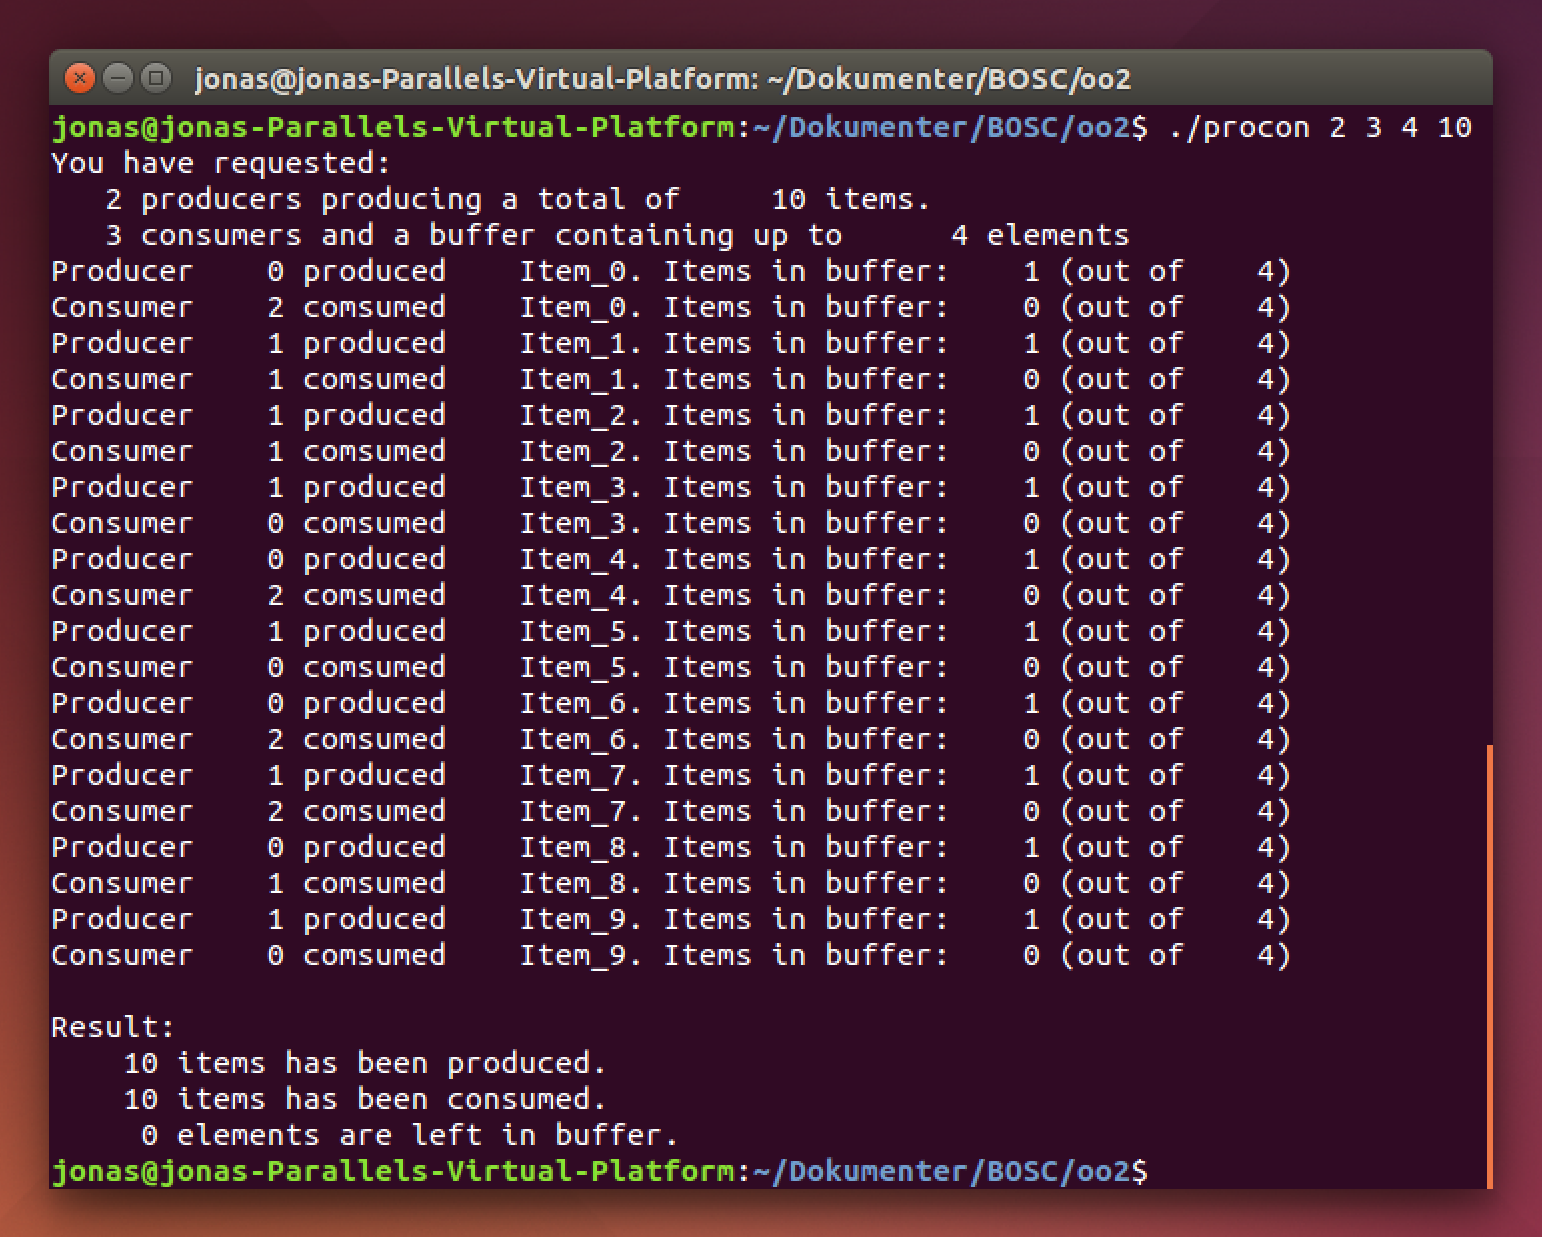
\includegraphics[width=0.95\textwidth]{opg3_test.png}}
\caption{Udskrift af eksekvering med 2 producenter, 3 forbrugere, buffer kapacitet på 4 og et total antal elementer på 10.}
\label{fig:opg2_2_test}
\end{figure}

\end{document}